\documentclass[dvipdfmx]{beamer}
\usetheme[
    block=fill, % ブロックに背景をつける
    progressbar=foot, % 各スライドの下にプログレスバー
    numbering=fraction % 合計ページ数を表示
]{metropolis}           % Use metropolis theme
\usepackage{float}
\usepackage{booktabs}
\usepackage{ascmac}
\usepackage{fancybox}
\usepackage{amsmath}
\usepackage{mathtools}
\usepackage{tikz}
\usetikzlibrary {arrows.meta}
\usetikzlibrary {bending}
\usepackage{listings,jvlisting} %日本語のコメントアウトをする場合jvlisting(もしくはjlisting)が必要
%ここからソースコードの表示に関する設定
\lstset{
  basicstyle={\ttfamily},
  identifierstyle={\small},
  commentstyle={\smallitshape},
  keywordstyle={\small\bfseries},
  ndkeywordstyle={\small},
  stringstyle={\small\ttfamily},
  frame={tb},
  breaklines=true,
  columns=[l]{fullflexible},
  numbers=left,
  xrightmargin=0zw,
  xleftmargin=3zw,
  numberstyle={\scriptsize},
  stepnumber=1,
  numbersep=1zw,
  lineskip=-0.5ex
}

\title{Progress}
\date{\today}
\author{Mizuno Yasuaki}
%\institute{Centre for Modern Beamer Themes}
\begin{document}
  \maketitle

  \begin{frame}{目次}
    \begin{enumerate}
      \item アミノ酸配列の画像作成
      \item 畳み込みニューラルネットワークによる学習
      \item k分割交差検証
      \item まとめ
    \end{enumerate}
  \end{frame}

  \begin{frame}{アミノ酸の画像作成}
    \begin{table}[H]
      \centering
      \caption{アミノ酸配列のベクトル割り当て①}
      \label{tab:amino_vector}
      \begin{tabular}{crrcrr}
        \toprule 
        アミノ酸 & x成分 & y 成分 & アミノ酸 & x成分 & y 成分 \\
        \midrule
        A & 2.5 & 1.10 & M & 6.0 & 1.90 \\
        C & 3.0 & 2.50 & N & 5.0 & -3.50 \\
        D & 2.5 & -3.60 & P & 5.5 & -1.90 \\ 
        E & 5.0 & -3.20 & Q & 6.0 & -3.68 \\
        F & 2.5 & 2.80 & R & 7.5 & -5.10 \\
        G & 0.5 & -3.68 & S & 3.0 & -0.50 \\
        H & 6.0 & -3.20 & T & 5.0 & 0.70 \\
        I & 5.5 & 4.50 & V & 5.0 & -0.46 \\
        L & 5.5 & 3.80 & Y & 7.0 & -1.30 \\
        \bottomrule
      \end{tabular}
    \end{table}
  \end{frame}

  \begin{frame}
    \begin{figure}[H]
      \centering
      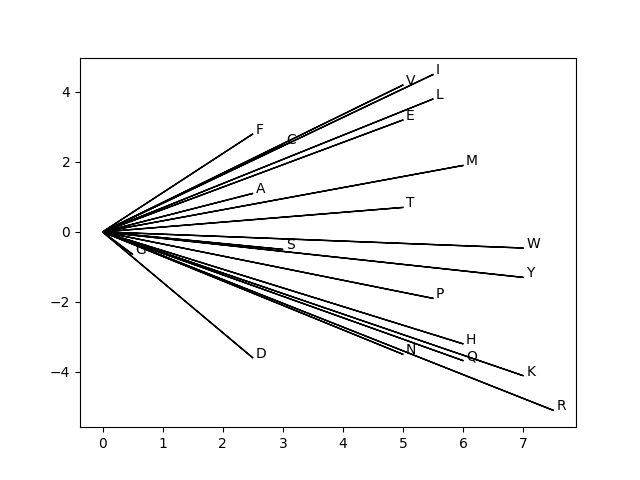
\includegraphics[keepaspectratio, scale=0.6]{images/amino_vector.png}
      \caption{アミノ酸のベクトル割り当て①}
      \label{fig:amino_vector}
    \end{figure}
  \end{frame}

  \begin{frame}
    Test Accuracy: 0.9507
    \begin{figure}
      \centering
      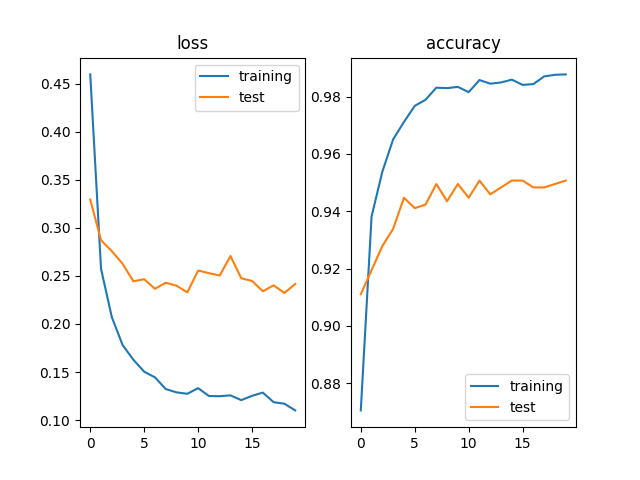
\includegraphics[keepaspectratio, scale=0.6]{images/train_fnn_amino_img.png}
      \caption{学習結果}
      \label{fig:result_amino_img}
    \end{figure}
  \end{frame}

  \begin{frame}{アミノ酸配列の画像作成}
    アミノ酸の疎水性度の最大値\(h_{max}\)と最小値\(h_{min}\)に対する角度をそれぞれ\(\theta_{max}\)と\(\theta_{min}\)と置く。
    \begin{figure}[H]
      \centering
      \begin{tikzpicture}
        % 軸
        \draw[->, >=stealth, semithick](-3,0)--(3,0)node[above]{$h$};
        \draw[->, >=stealth, semithick](0, -1)--(0, 3)node[right]{$\theta$};

        % 点の定義
        \fill (0, 0) coordinate (O) circle[radius=2pt] node[below left] {O};
        \fill (-2, 2) coordinate (A) circle[radius=2pt] node[left=2pt] {$(h_{min}, \theta_{min})$};
        \fill (2, 1) coordinate (B) circle[radius=2pt] node[right=2pt] {$(h_{max}, \theta_{max})$};
        
        % 直線の描写
        \draw (A)--(B);
      \end{tikzpicture}
    \end{figure}
  \end{frame}

  \begin{frame}
    任意のアミノ酸の疎水性度を\(h_{amino}\)、角度を\(\theta_{amino}\)とすると
    \begin{equation}
      \label{eq:calc_amino}
      \theta_{amino} = \frac{\theta_{max} - \theta_{min}}{h_{max} - h_{min}} d\times (h_{amino} - h_{max}) + \theta_{max}
    \end{equation}
    となる。\((h_{max}, \theta_{max}) = (4.50, 10)\)と\((h_{min}, \theta_{min}) = (-5.10, 170)\)をそれぞれ式(\ref{eq:calc_amino})に代入する。
    \begin{equation}
      \label{eq:calc_amino_concreate}
      \theta_{amino} = \frac{50}{3} \times h_{amino} + 85
    \end{equation}
  \end{frame}

  \begin{frame}
    \begin{table}[H]
      \centering
      \caption{アミノ酸の角度割り当て②}
      \label{tab:amino_theta}
      \begin{tabular}{crrcrr}
        \toprule
        アミノ酸 & 疎水性度 & $\theta$ & アミノ酸 & 疎水性度 & $\theta$ \\
        \midrule
        R & -5.10 & 170.0 & G & -0.64 & 95.6 \\
        K & -4.11 & 153.5 & S & -0.50 & 93.3 \\
        Q & 3.68 & 23.6 & W & -0.46 & 92.6 \\
        D & -3.60 & 145.0 & A & 1.10 & 66.6 \\
        N & -3.50 & 143.3 & M & 1.90 & 53.3 \\
        H & -3.20 & 138.3 & C & 2.50 & 43.3 \\
        E & -3.20 & 138.3 & F & 2.80 & 38.3 \\
        P & -1.90 & 116.6 & L & 3.80 & 21.6 \\
        Y & -1.30 & 106.6 & V & 4.20 & 14.9 \\
        T & 0.70 & 73.3 & I & 4.50 & 10.0 \\
        \bottomrule
      \end{tabular}
    \end{table}
  \end{frame}

  \begin{frame}
    疎水性度に同じ値があるので、アミノ酸のベクトル割り当て①のようにアミノ酸の大きさの情報を加える。
    アミノ酸の大きさを\(r_{amino}\)とすると、極座標を用いて
    \begin{equation}
      (r_{amino}, \theta_{amino})
    \end{equation}
    と表すことができる。
  \end{frame}

  \begin{frame}
    \begin{figure}[H]
      \centering
      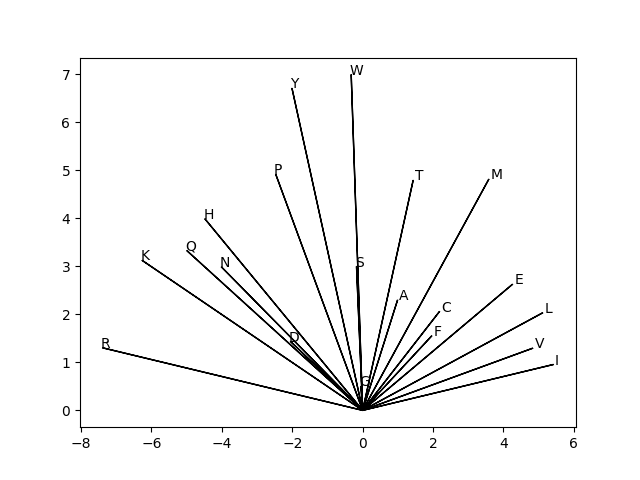
\includegraphics[keepaspectratio, scale=0.6]{images/my_amino_vector.png}
      \caption{アミノ酸のベクトル割り当て②}
      \label{fig:my_amino_vector}
    \end{figure}
  \end{frame}

  \begin{frame}{アミノ酸配列の画像比較}
    \begin{figure}[htbp]
      \begin{minipage}[b]{0.45\linewidth}
        \centering
        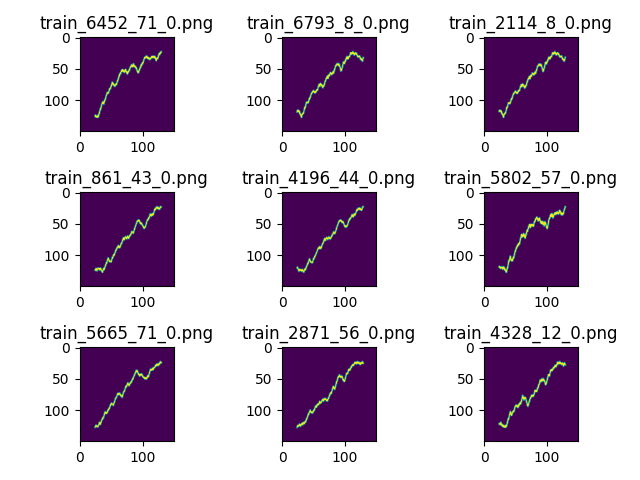
\includegraphics[keepaspectratio, scale=0.3]{images/amino_img_classA.png}
        \caption{\newline ベクトル①を用いた画像}
      \end{minipage}
      \begin{minipage}[b]{0.45\linewidth}
        \centering
        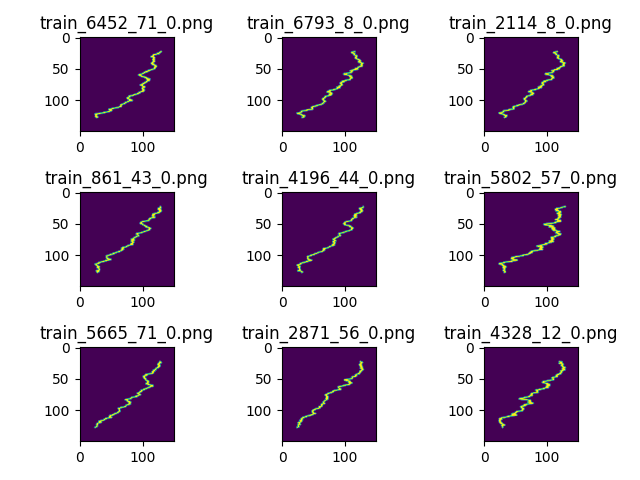
\includegraphics[keepaspectratio, scale=0.3]{images/my_amino_img_classA.png}
        \caption{\newline ベクトル②を用いた画像}
      \end{minipage}
    \end{figure}
  \end{frame}

  \begin{frame}
    Test Accuracy: 0.9519
    \begin{figure}[H]
      \centering
      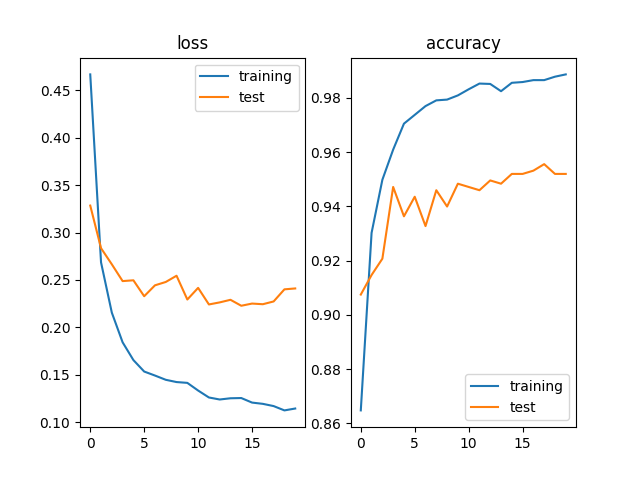
\includegraphics[keepaspectratio, scale=0.6]{images/train_fnn_my_amino_img.png}
    \end{figure}
  \end{frame}

  \begin{frame}{畳み込みニューラルネットワークによる学習}
    \begin{block}{単純な畳み込みニューラルネットワークのモデル}
      \begin{itemize}
        \item 畳み込み層 \mbox{}\\チャンネル数:32、フィルタサイズ:(3, 3)、活性化関数:Relu
        \item マックスプーリング層 \mbox{}プーリングサイズ:(2, 2)
        \item Flatten層
        \item ドロップアウト層 \mbox{}ドロップアウト率:0.3
        \item 全結合層 \mbox{}ノード数:32、活性化関数:Relu
        \item 出力層 \mbox{}ノード数:5、活性化関数:softmax
        \item バッチサイズ:128
        \item エポック:10
      \end{itemize}
    \end{block}
  \end{frame}

  \begin{frame}
    \begin{figure}[htbp]
      \begin{minipage}[b]{0.45\linewidth}
        \centering
        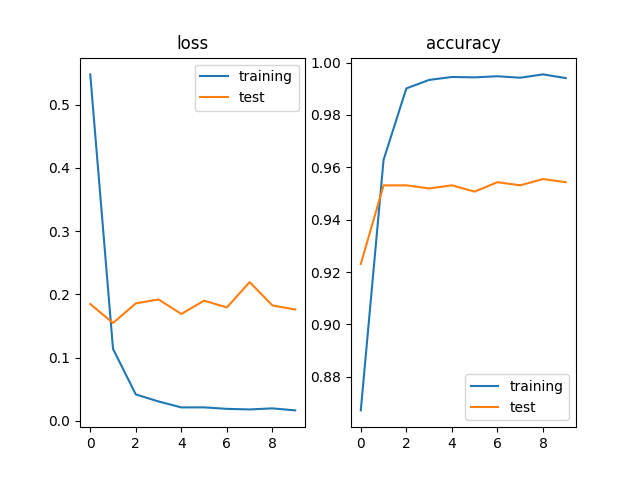
\includegraphics[keepaspectratio, scale=0.3]{images/train_cnn_amino_img.png}
        \caption{\newline アミノ酸配列画像①の学習結果 \newline Accuracy: 0.9543}
      \end{minipage}
      \begin{minipage}[b]{0.45\linewidth}
        \centering
        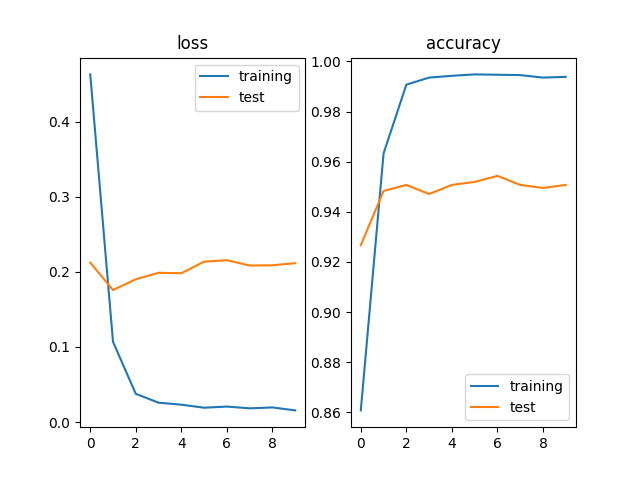
\includegraphics[keepaspectratio, scale=0.3]{images/train_cnn_my_amino_img.png}
        \caption{\newline アミノ酸配列画像②の学習結果 \newline Accuracy: 0.9507}
      \end{minipage}
    \end{figure}
  \end{frame}

  \begin{frame}{k分割交差検証}
    \begin{itemize}
        \item 訓練データを同じサイズのk個のサブセットに分ける
        \item (k - 1)個のサブセットで訓練し、残りのサブセットで評価する
        \item 最終的にk個のスコアの平均
    \end{itemize}
  \end{frame}

  \begin{frame}
    \begin{figure}
      \centering
      \begin{tikzpicture}
        % 一列目
        \draw [fill=yellow, rounded corners=10pt] (0, 3)rectangle(2, 4) (1, 3.5)node{検証};
        \draw [rounded corners=10pt] (2.5, 3)rectangle(4.5, 4) (3.5, 3.5)node{訓練};
        \draw [rounded corners=10pt] (5, 3)rectangle(7, 4) (6, 3.5)node{訓練};
        \draw [->] (7.5, 3.5)--(8, 3.5) node[right]{検証スコア①};
        % 二列目
        \draw [rounded corners=10pt] (0, 1.5)rectangle(2, 2.5) (1, 2)node{訓練};
        \draw [fill=yellow, rounded corners=10pt] (2.5, 1.5)rectangle(4.5, 2.5) (3.5, 2)node{検証};
        \draw [rounded corners=10pt] (5, 1.5)rectangle(7, 2.5) (6, 2)node{訓練};
        \draw [->] (7.5, 2)--(8, 2) node[right]{検証スコア②};
        % 三列目
        \draw [rounded corners=10pt] (0, 0)rectangle(2, 1) (1, .5)node{訓練};
        \draw [rounded corners=10pt] (2.5, 0)rectangle(4.5, 1) (3.5, .5)node{訓練};
        \draw [fill=yellow, rounded corners=10pt] (5, 0)rectangle(7, 1) (6, .5)node{検証};
        \draw [->] (7.5, .5)--(8, .5) node[right]{検証スコア③};
      \end{tikzpicture}
      \caption{3分割交差検証}
    \end{figure}
  \end{frame}

  \begin{frame}{k分割交差検証結果}
    \begin{table}[H]
      \centering
      \caption{4分割交差検証}
      \begin{tabular}{crr}
        \hline
        フォールド & アミノ酸配列の画像① & アミノ酸配列の画像② \\
        \hline \hline
        0 & 0.9483 & 0.9447 \\
        1 & 0.9350 & 0.9507 \\
        2 & 0.9531 & 0.9579 \\
        3 & 0.9555 & 0.9519 \\
        \hline
        Average & 0.9480 & 0.9513 \\
        \hline
      \end{tabular}
    \end{table}
  \end{frame}

  \begin{frame}{まとめ}
    \begin{itemize}
      \item 画像やニューラルネットワークを変更してみたがあまり精度は変わらなかった
      \item 交差検証をテストケースでおこなう
      \item 以前読んだ論文で使用されていたAttention層やRNN層を用いて精度を向上させる
    \end{itemize}
  \end{frame}

\end{document}


